\chapter{Results}
\label{chap:resultados}

This chapter presents the experimental results of the HoTHP in two contexts: synthetic data, where the generating process is known, and real data, where it is not. Next, we visualize the intensities learned by the models to understand the behavior of the recency bias in practice, and we run an ablation to isolate the effect of the temporal scale.

\section{Synthetic data}
\label{sec:resultados-sinteticos}

The synthetic experiments follow the protocol described in Section~\ref{sec:configuracao-experimental}, using Hawkes processes with an exponential kernel in the slow decay ($\beta$ small) and fast decay ($\beta$ large) scenarios. We compare four models: NHP, THP, RoTHP, and HoTHP. Table~\ref{tab:resultados-sinteticos} summarizes the results for the \textit{train short, test long} protocol, varying the extrapolation factor $\alpha$ from $1\times$ (training length) to $10\times$. Figure~\ref{fig:extrapolacao-sintetica} visualizes the evolution of the NLL as a function of $\alpha$.

\begin{table}[h!]
\centering
\caption{NLL (mean $\pm$ standard deviation, 10 seeds) on the synthetic data. Lower values indicate better performance. The best result for each configuration is in bold.}
\label{tab:resultados-sinteticos}
\resizebox{\textwidth}{!}{%
\begin{tabular}{llcccc}
\toprule
Scenario & Model & $1\times$ & $2\times$ & $5\times$ & $10\times$ \\
\midrule
\multirow{4}{*}{Slow decay}
    & NHP    & $\mathbf{1{,}470 \pm 0{,}007}$ & $2{,}197 \pm 0{,}131$ & $2{,}667 \pm 0{,}236$ & $2{,}817 \pm 0{,}273$ \\
    & THP    & $1{,}475 \pm 0{,}007$ & $3{,}926 \pm 1{,}505$ & $4{,}127 \pm 1{,}803$ & $4{,}199 \pm 2{,}117$ \\
    & RoTHP  & $1{,}499 \pm 0{,}014$ & $2{,}007 \pm 0{,}284$ & $2{,}642 \pm 0{,}509$ & $3{,}001 \pm 0{,}625$ \\
    & HoTHP  & $1{,}545 \pm 0{,}025$ & $\mathbf{1{,}609 \pm 0{,}096}$ & $\mathbf{1{,}943 \pm 0{,}313}$ & $\mathbf{2{,}364 \pm 0{,}625}$ \\
\midrule
\multirow{4}{*}{Fast decay}
    & NHP    & $\mathbf{1{,}663 \pm 0{,}005}$ & $1{,}833 \pm 0{,}134$ & $2{,}057 \pm 0{,}223$ & $2{,}153 \pm 0{,}250$ \\
    & THP    & $1{,}677 \pm 0{,}011$ & $3{,}391 \pm 0{,}781$ & $3{,}761 \pm 1{,}072$ & $3{,}897 \pm 1{,}509$ \\
    & RoTHP  & $1{,}681 \pm 0{,}007$ & $2{,}039 \pm 0{,}279$ & $2{,}146 \pm 0{,}309$ & $2{,}275 \pm 0{,}372$ \\
    & HoTHP  & $1{,}689 \pm 0{,}008$ & $\mathbf{1{,}701 \pm 0{,}012}$ & $\mathbf{1{,}740 \pm 0{,}050}$ & $\mathbf{1{,}774 \pm 0{,}092}$ \\
\bottomrule
\end{tabular}
}
\end{table}

\begin{figure}[h!]
    \centering
    \captionsetup{width=14cm}
    \Caption{\label{fig:extrapolacao-sintetica} NLL (mean $\pm$ standard deviation, 10 seeds) as a function of the extrapolation factor $\alpha$ in the synthetic scenarios. The HoTHP keeps the NLL more stable as $\alpha$ grows, while the THP degrades drastically and the RoTHP and NHP show intermediate degradation.}
    \UFCfig{}{
        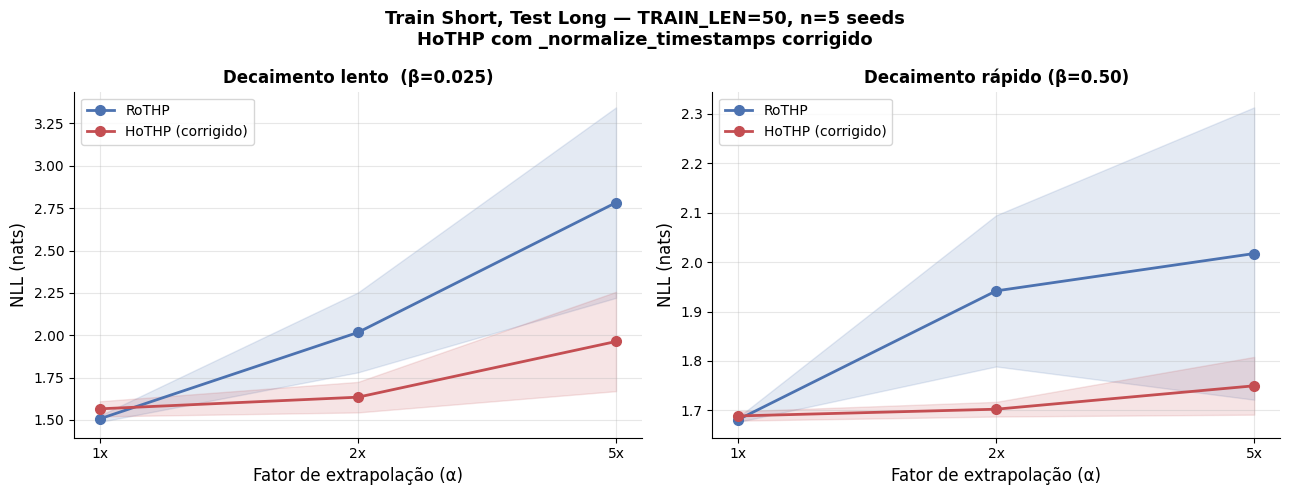
\includegraphics[width=14cm]{figuras/fig_extrapolation_nll_sintetico.png}
    }{
    }
\end{figure}

With the inclusion of the NHP and the THP as baselines, four distinct behaviors emerge in the extrapolation. The THP is the model that degrades the most: its NLL jumps to $\approx 3{,}9$ already at $2\times$ and stays between $\approx 3{,}9$ and $\approx 4{,}2$ at the larger factors, in both scenarios, with a very high standard deviation (up to $\pm 2{,}12$) caused by seeds that diverge completely. This confirms that the absolute temporal encoding of the THP produces representations outside the distribution for new positions. The NHP, despite not using attention, is the most competitive baseline in the extrapolation, probably because its recurrent architecture accumulates information incrementally, without depending on absolute positions; even so, it stays behind the HoTHP at all extrapolation factors in both scenarios.

The HoTHP obtains the best NLL at all extrapolation factors ($2\times$, $5\times$, and $10\times$) in both scenarios. The cost of this advantage appears in distribution: at $1\times$, the HoTHP is the model with the worst NLL (for example, $1{,}545$ against $1{,}470$ of the NHP in the slow decay), a small difference that reverses as soon as the test sequence goes beyond the training length. In the fast decay, the NLL of the HoTHP grows by only $0{,}085$ between $1\times$ and $10\times$ ($1{,}689 \to 1{,}774$), staying practically flat, while the second best model (NHP) grows by $0{,}490$ ($1{,}663 \to 2{,}153$). This stability is expected: since the generating process has an exponential kernel, the recency bias of the HoTHP is perfectly aligned with the real structure of the data. For temporal distances not seen in training, the hyperbolic kernel keeps decaying monotonically, while the trigonometric kernel of the RoTHP oscillates in phases that were not learned and the absolute encoding of the THP diverges.

The advantage of the HoTHP over the three baselines is statistically significant (Wilcoxon signed-rank test, paired by seed and one-sided, $p < 0{,}05$) at all extrapolation factors of both scenarios, without exception. The least comfortable case is the slow decay at $10\times$ against the NHP ($p = 0{,}042$); in all the other comparisons the $p$-value is $0{,}025$ or below, reaching the floor of $0{,}001$ (equal to $1/2^{10}$, the smallest possible value for the one-sided test with 10 seeds) in most of them.

In the slow decay, where the influence of distant events persists for longer, the HoTHP still obtains the best mean NLL at all factors, but its degradation is much larger than in the fast decay: the NLL grows by $0{,}819$ between $1\times$ and $10\times$, against only $0{,}085$ in the fast decay. At $10\times$, the mean of the HoTHP ($2{,}364$) is lower than that of the NHP ($2{,}817$) and the difference remains statistically significant, even if by the narrowest margin of the whole experiment ($p = 0{,}042$), reflecting the high variance between seeds in this regime ($\pm 0{,}625$). This suggests that, when the memory of the process is long, the exponential decay imposed by the hyperbolic kernel may discard events that are still relevant too early, reducing the advantage margin.

Figure~\ref{fig:extrapolacao-rmse} shows the RMSE of the next event prediction. In the slow decay, all the models degrade in a similar way (RMSE $\approx 2{,}7$--$2{,}8$ at $10\times$), with the HoTHP showing the lowest RMSE ($2{,}714$). In the fast decay, the four models keep a stable and close RMSE (between $\approx 1{,}40$ and $1{,}55$ at $10\times$): the RoTHP obtains the lowest value ($1{,}407$) and the NHP the highest ($1{,}549$), the latter with a slightly higher variance due to an atypical seed. Unlike the NLL, the RMSE does not separate the models clearly. This indicates that the advantage of the HoTHP shows up mainly in the likelihood, that is, in modeling the full temporal distribution, and not in the pointwise prediction of the next interval, where the attention models are practically tied.

\begin{figure}[h!]
    \centering
    \captionsetup{width=14cm}
    \Caption{\label{fig:extrapolacao-rmse} RMSE of the next event prediction (mean $\pm$ standard deviation, 10 seeds) as a function of the extrapolation factor $\alpha$. Unlike the NLL, the RMSE does not separate the models clearly: in the slow decay all of them degrade in a similar way and in the fast decay they stay close to each other.}
    \UFCfig{}{
        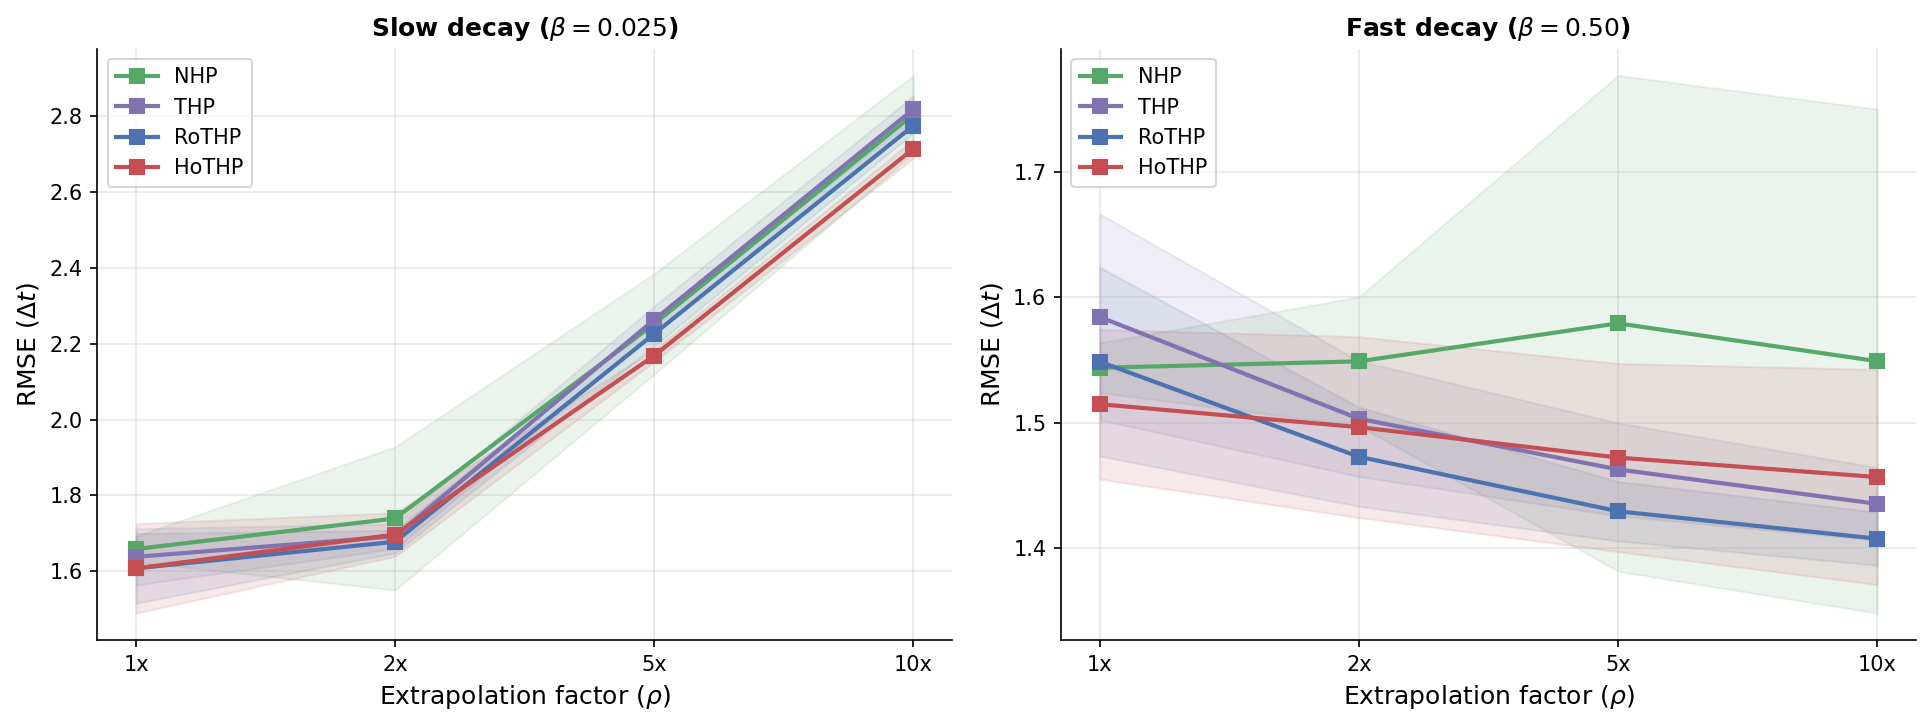
\includegraphics[width=14cm]{figuras/fig_extrapolation_rmse_sintetico.png}
    }{
    }
\end{figure}

\section{Real data}
\label{sec:resultados-reais}

To evaluate the HoTHP in more realistic scenarios, we ran experiments on four public point process datasets. Table~\ref{tab:datasets-reais} describes each dataset.

\begin{table}[h!]
\centering
\caption{Real datasets used in the experiments. $L_{\text{train}}$ is the maximum training length (number of events) and $L_{5\times}$ is the test length in the extrapolation condition.}
\label{tab:datasets-reais}
\begin{tabular}{lccccc}
\toprule
Dataset & Types & Sequences (train) & $L_{\text{train}}$ & $L_{5\times}$ & Domain \\
\midrule
Amazon         & 16 & 6.454  & 18 & 90  & Product reviews \\
Stackoverflow  & 22 & 1.401  & 20 & 100 & User badges \\
Taxi           & 10 & 1.400  &  7 & 38  & Taxi rides \\
Retweet        &  3 & 20.000 & 50 & 250 & Retweet cascades \\
\bottomrule
\end{tabular}
\end{table}

We follow the same \textit{train short, test long} protocol: we train each model with sequences truncated at $L_{\text{train}}$ events and evaluate both at the training length ($1\times$) and at extrapolation ($5\times$). We use three seeds (2019, 2020, 2021), 100 epochs, and the same hyperparameters as in Section~\ref{subsec:modelos-comparados}. For Amazon and Stackoverflow, we compare THP, RoTHP, and HoTHP; for Taxi and Retweet, we compare only RoTHP and HoTHP.

Table~\ref{tab:resultados-reais} presents the results.

\begin{table}[h!]
\centering
\caption{NLL on the real datasets (mean $\pm$ standard deviation, 3 seeds). $\Delta$NLL is the difference $5\times$ minus $1\times$: negative values indicate that the model improves with longer sequences. Lower NLL values are better. The best result for each dataset and condition is in bold.}
\label{tab:resultados-reais}
\resizebox{\textwidth}{!}{%
\begin{tabular}{llcccc}
\toprule
Dataset & Model & NLL $1\times$ & NLL $5\times$ & $\Delta$NLL & Acc $5\times$ \\
\midrule
\multirow{3}{*}{Amazon}
    & THP    & $2{,}274 \pm 0{,}002$ & $2{,}244 \pm 0{,}007$ & $-0{,}030$ & $0{,}322 \pm 0{,}004$ \\
    & RoTHP  & $2{,}272 \pm 0{,}004$ & $2{,}252 \pm 0{,}002$ & $-0{,}020$ & $0{,}321 \pm 0{,}004$ \\
    & HoTHP  & $2{,}268 \pm 0{,}002$ & $\mathbf{2{,}194 \pm 0{,}002}$ & $\mathbf{-0{,}074}$ & $\mathbf{0{,}340 \pm 0{,}002}$ \\
\midrule
\multirow{3}{*}{Stackoverflow}
    & THP    & $2{,}745 \pm 0{,}011$ & $\mathbf{2{,}521 \pm 0{,}020}$ & $-0{,}224$ & $0{,}451 \pm 0{,}002$ \\
    & RoTHP  & $2{,}753 \pm 0{,}005$ & $2{,}538 \pm 0{,}003$ & $-0{,}215$ & $0{,}450 \pm 0{,}000$ \\
    & HoTHP  & $2{,}742 \pm 0{,}020$ & $2{,}530 \pm 0{,}023$ & $-0{,}212$ & $0{,}451 \pm 0{,}003$ \\
\midrule
\multirow{2}{*}{Taxi}
    & RoTHP  & $-0{,}269 \pm 0{,}005$ & $-0{,}176 \pm 0{,}041$ & $+0{,}092$ & $0{,}907 \pm 0{,}002$ \\
    & HoTHP  & $-0{,}271 \pm 0{,}006$ & $\mathbf{-0{,}212 \pm 0{,}009}$ & $\mathbf{+0{,}059}$ & $0{,}907 \pm 0{,}003$ \\
\midrule
\multirow{2}{*}{Retweet}
    & RoTHP  & $12{,}5 \pm 4{,}9$ & $\mathbf{121 \times 10^3}$ & --- & $0{,}520 \pm 0{,}042$ \\
    & HoTHP  & $12{,}5 \pm 4{,}8$ & $367 \times 10^3$ & --- & $0{,}518 \pm 0{,}039$ \\
\bottomrule
\end{tabular}
}
\end{table}

Three distinct patterns emerge from the results:

\textbf{Amazon: HoTHP wins.} The HoTHP obtains the best NLL in both conditions and shows the largest gain in extrapolation ($\Delta\text{NLL} = -0{,}074$, against $-0{,}020$ of the RoTHP). The difference is small in absolute value, but consistent across the three seeds (standard deviation of $0{,}002$).

\textbf{Stackoverflow: tie.} The three models show practically identical NLL at $5\times$, with differences within the margin of error. No model benefits more than the others from longer sequences. This suggests that the dataset does not have a temporal structure that differentiates the positional biases of the three models.

\textbf{Taxi: tie with a slight advantage for the HoTHP.} The HoTHP degrades less in extrapolation ($\Delta\text{NLL} = +0{,}059$ against $+0{,}092$ of the RoTHP), but the difference is modest and the variance of the RoTHP is high.

\textbf{Retweet: both models fail.} The NLL at $5\times$ explodes to values on the order of $10^5$, with the HoTHP worse than the RoTHP ($367 \times 10^3$ against $121 \times 10^3$). The extreme temporal scale of this dataset (intervals between events of up to 582.928 time units) makes the hyperbolic kernel saturate numerically, as discussed in Section~\ref{sec:estabilidade-numerica}.

\subsection{Training convergence}
\label{subsec:convergencia}

Figure~\ref{fig:convergencia} shows the convergence curves of the validation NLL over the 100 training epochs. On the Amazon and Stackoverflow datasets, the three models converge smoothly, with the NLL stabilizing after epoch 50. On Amazon, the curve still shows a slight downward trend in the last 20 epochs, but with a slope below $0{,}01$ per epoch, which indicates that additional epochs would benefit all the models equally without changing the ranking.

On Taxi, the RoTHP shows higher variance between seeds in the early epochs (10 to 40), but converges to the same level as the HoTHP after epoch 40. On Retweet, the convergence reveals the numerical collapse: 2 out of 3 seeds stabilize at NLL $\approx 15{,}9$, while only one seed (2019) converges to informative values ($\text{NLL} \approx 5{,}5$). The resulting standard deviation band is enormous, visually confirming the instability reported in Table~\ref{tab:resultados-reais}.

\begin{figure}[h!]
    \centering
    \captionsetup{width=14cm}
    \Caption{\label{fig:convergencia} Convergence curves of the validation NLL (mean $\pm$ standard deviation, 3 seeds). The first epochs were omitted to improve the visualization. On Amazon and Stackoverflow, all the models converge smoothly. On Taxi, the RoTHP is more unstable in the early epochs. On Retweet, the wide band of the RoTHP reflects the collapse of 2 of the 3 seeds.}
    \UFCfig{}{
        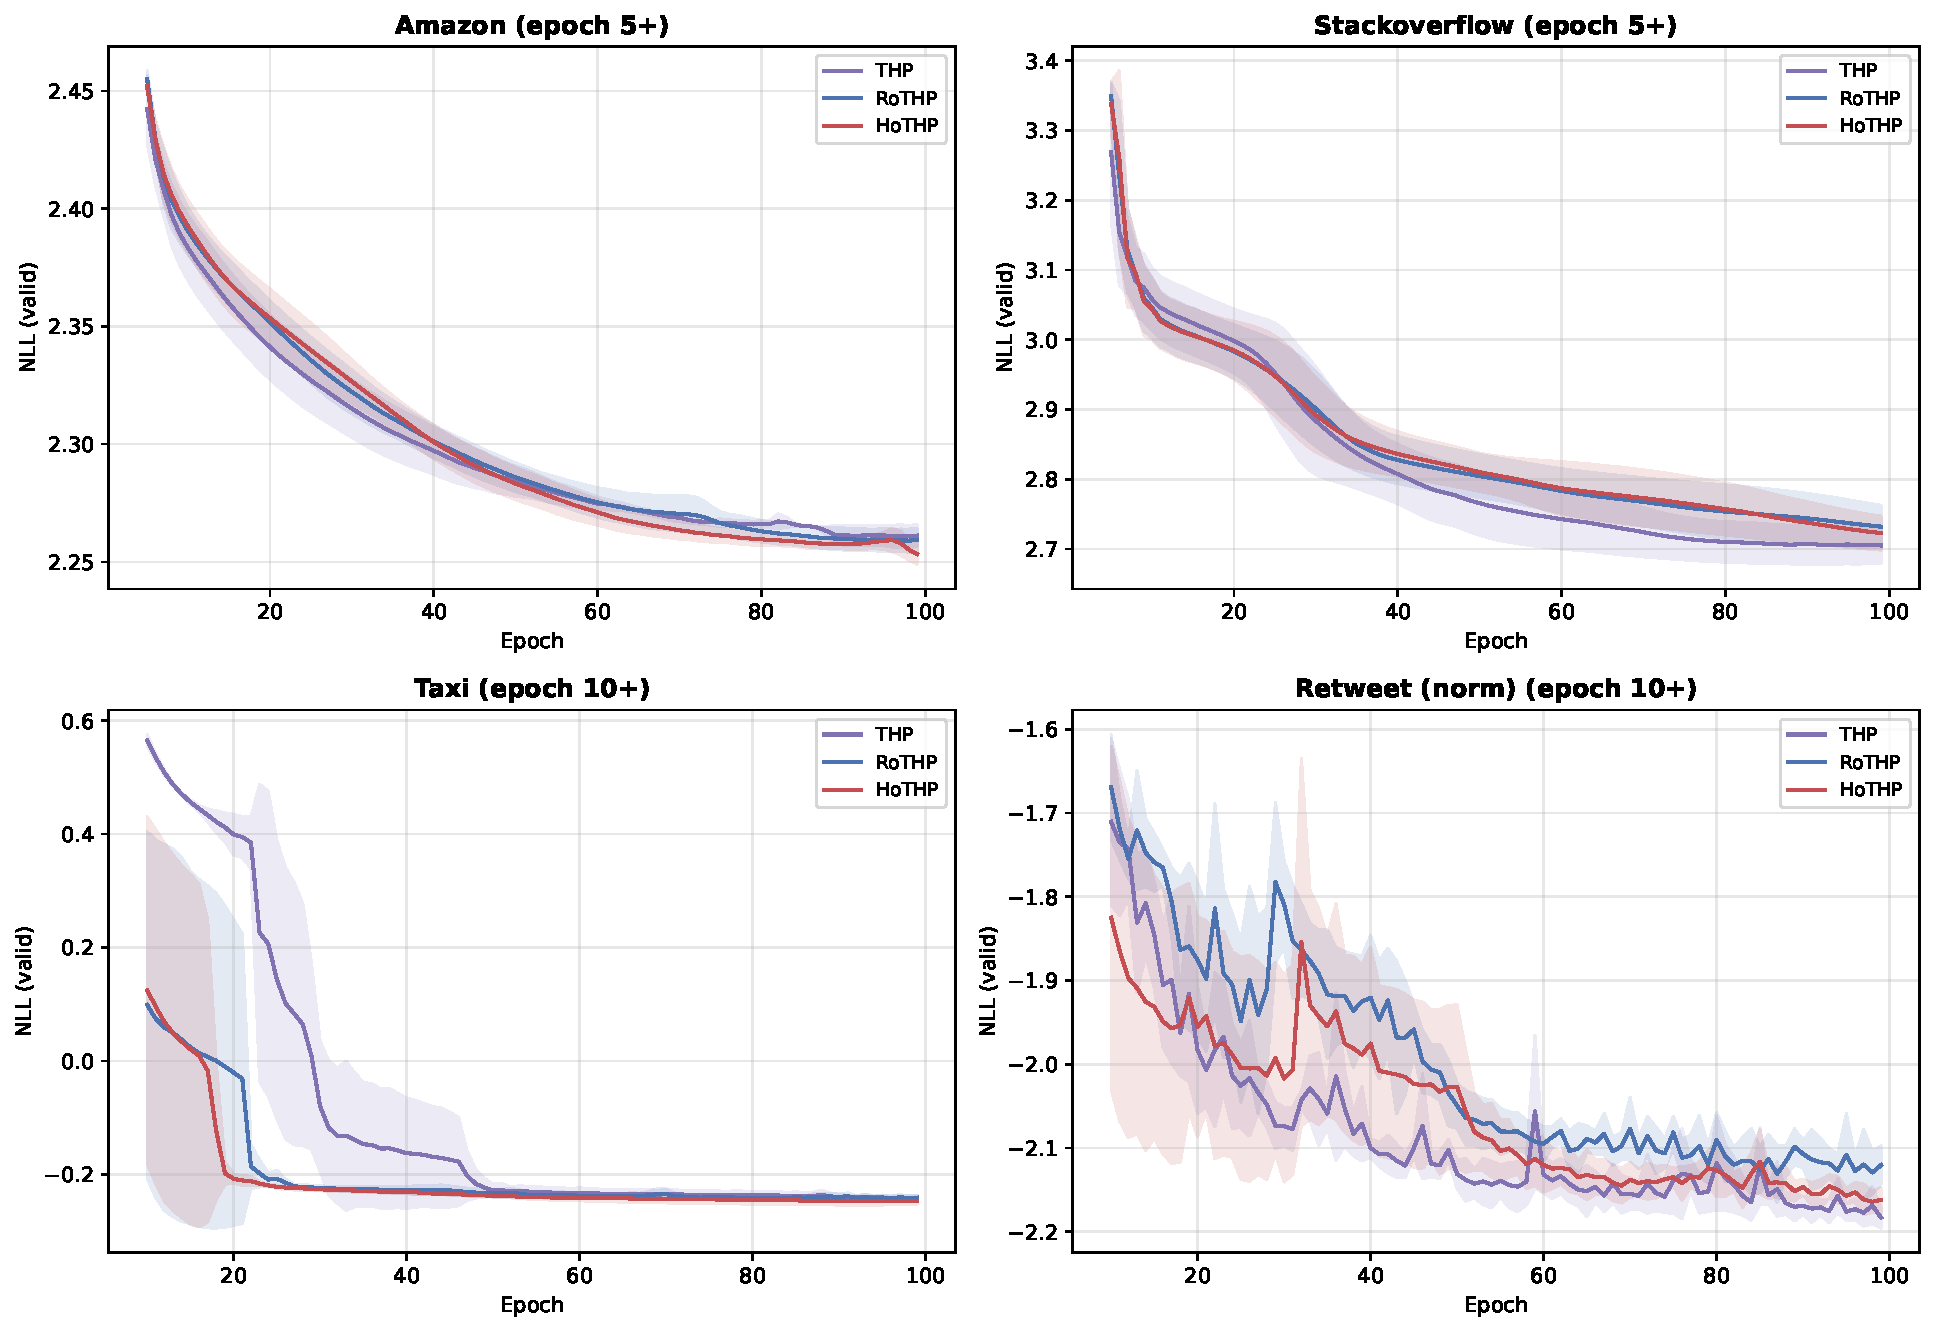
\includegraphics[width=14cm]{figuras/fig_convergencia.pdf}
    }{
    }
\end{figure}

\section{Intensities learned by the models}
\label{sec:intensidades-aprendidas}

To understand why the HoTHP behaves differently on each dataset, we extracted the conditional intensity function $\lambda^*(t)$ that each trained model computes for representative test sequences. Figure~\ref{fig:intensidades} shows the total intensity $\lambda^*(t) = \sum_k \lambda_k^*(t)$ over time for the Amazon, Stackoverflow, and Retweet datasets.

\begin{figure}[h!]
    \centering
    \captionsetup{width=14cm}
    \Caption{\label{fig:intensidades} Conditional intensity $\lambda^*(t)$ learned by the THP (orange), RoTHP (blue), and HoTHP (green) for one test sequence of each dataset. The gray vertical bars indicate the events. On Amazon, the intensity grows between events and falls when an event occurs (self-inhibition). On Stackoverflow, the intensity is approximately constant (memoryless process). On Retweet, both models collapse to $\lambda^* \approx 0$ after the initial burst due to the extreme temporal scale.}
    \UFCfig{}{
        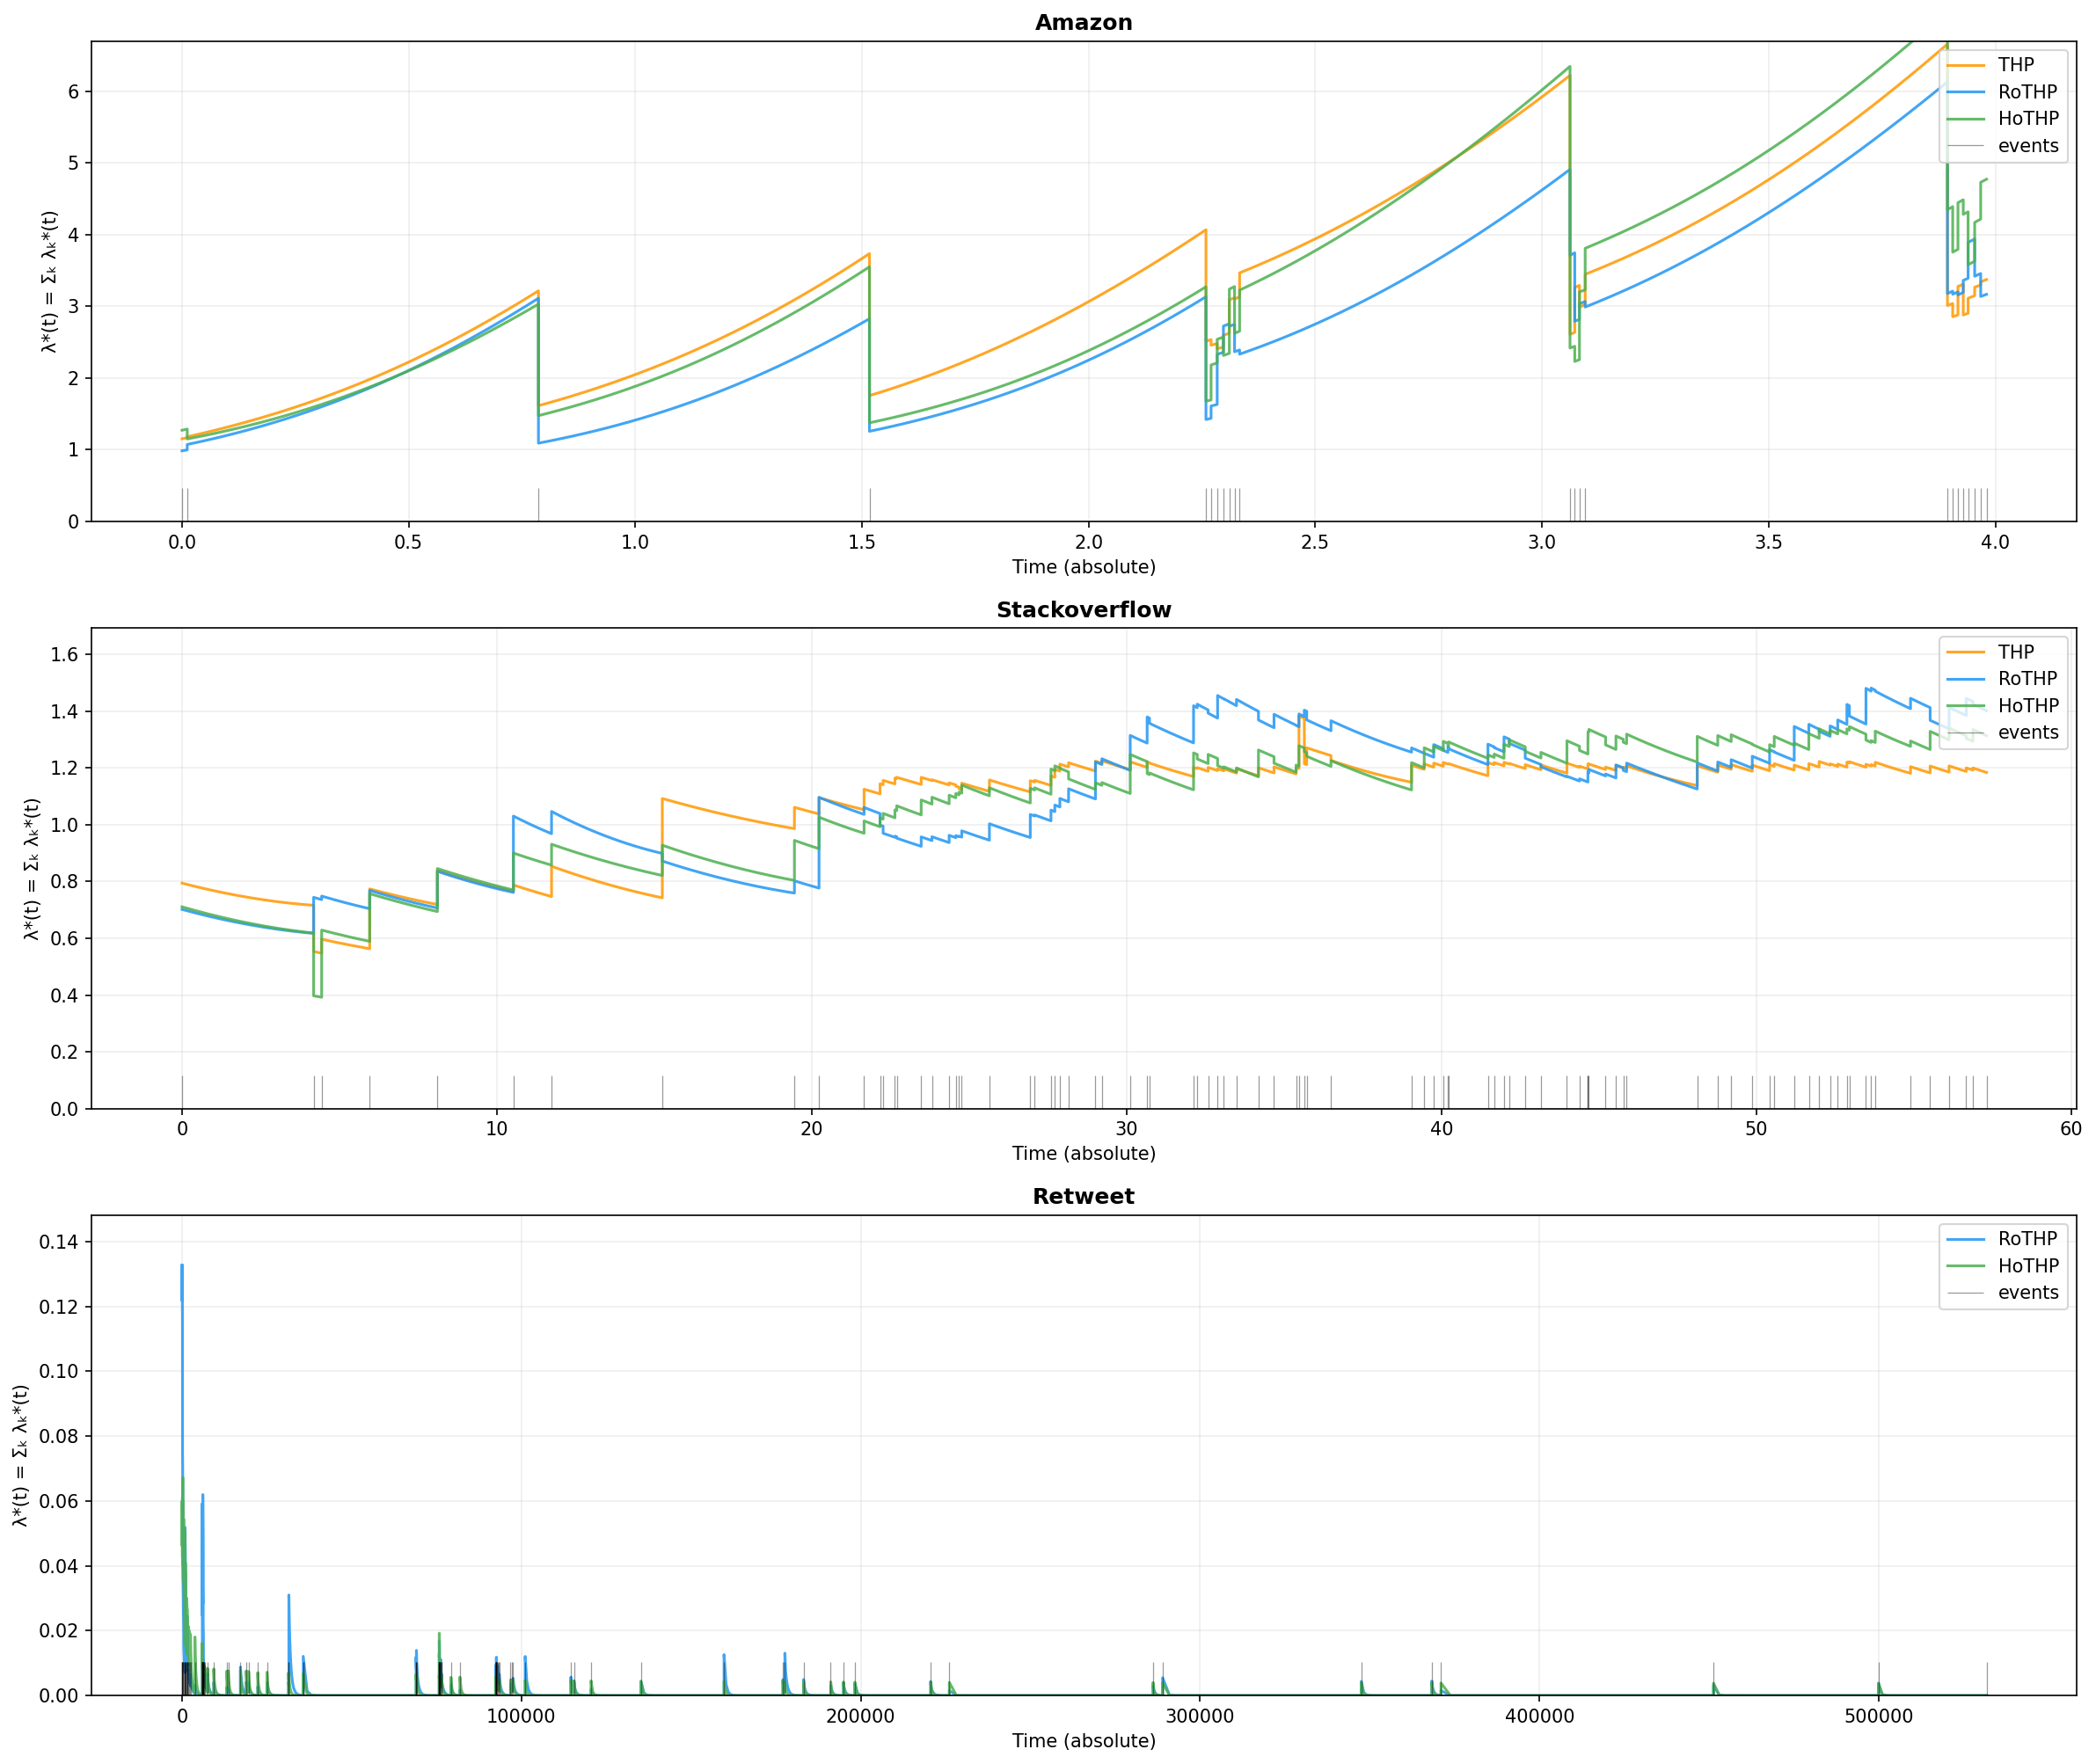
\includegraphics[width=14cm]{figuras/fig_model_intensity.png}
    }{
    }
\end{figure}

On Amazon, the intensity grows between events and falls when an event occurs, indicating that each event reduces the chance of new events in the short term. Even so, the most recent event is the most informative for the prediction, which explains why the recency bias of the HoTHP helps on this dataset. On Stackoverflow, the three models learn a practically flat intensity, with no visible reaction to the events, characteristic of a process with little temporal memory, and no positional bias manages to stand out. On Retweet, the models only react to the initial burst and then the intensity falls to practically zero, because the intervals between events are too large for any decay function.

The observation on Amazon is particularly relevant in light of Section~\ref{sec:onde-atua-vies}: the HoTHP wins on this dataset even though the process is self-inhibiting, not self-exciting. This confirms that the recency bias acts on the attention (``which past events are more relevant'') and not on the intensity (``the intensity rises or falls after an event''). On Amazon, the most recent event is the most informative for predicting the next one and the exponential decay in the attention captures this correctly.

\section{Ablation: temporal normalization of Retweet}
\label{sec:ablacao-retweet}

The numerical collapse observed on Retweet raises a question: is the problem the temporal scale or the HoTHP bias itself? To isolate these factors, we ran an ablation in which we normalize the Retweet timestamps before training.

The normalization consists of dividing all the instants of each sequence by the mean of the intervals of that sequence.

After this operation, the mean interval between events becomes approximately~1 in all the sequences, with the maximum interval reduced from~582.928 to approximately~227. The temporal structure (order of the events, clustering patterns, types) is preserved. Only the numerical scale changes.

We trained the RoTHP and the HoTHP on the normalized Retweet with the same hyperparameters (3 seeds, 100 epochs, $L_{\text{train}} = 50$, $L_{5\times} = 250$) and compared with the original results.

\begin{table}[h!]
\centering
\caption{Ablation: effect of the temporal normalization on Retweet. ``Original'' uses the raw timestamps; ``Normalized'' uses the timestamps divided by the mean of the gaps. Mean $\pm$ standard deviation (3 seeds).}
\label{tab:ablacao-retweet}
\begin{tabular}{llcccc}
\toprule
Version & Model & NLL $1\times$ & NLL $5\times$ & Acc $1\times$ & Acc $5\times$ \\
\midrule
\multirow{2}{*}{Original}
    & RoTHP  & $12{,}456 \pm 6{,}038$ & $1 \times 10^{5}$ & $0{,}496 \pm 0{,}072$ & $0{,}520 \pm 0{,}051$ \\
    & HoTHP  & $12{,}517 \pm 5{,}932$ & $4 \times 10^{5}$ & $0{,}495 \pm 0{,}071$ & $0{,}518 \pm 0{,}047$ \\
\midrule
\multirow{2}{*}{Normalized}
    & RoTHP  & $-2{,}197 \pm 0{,}163$ & $88{,}856 \pm 144{,}800$ & $0{,}588 \pm 0{,}036$ & $0{,}562 \pm 0{,}014$ \\
    & HoTHP  & $-2{,}168 \pm 0{,}010$ & $\mathbf{-0{,}542 \pm 0{,}004}$ & $0{,}591 \pm 0{,}002$ & $\mathbf{0{,}588 \pm 0{,}004}$ \\
\bottomrule
\end{tabular}
\end{table}

The normalization resolves the numerical collapse unambiguously. With raw timestamps, the NLL at $1\times$ is approximately $12{,}5$ for both models and the NLL at $5\times$ explodes to the order of $10^5$. With normalized timestamps, the NLL at $1\times$ drops to negative values and the training converges across all the seeds.

The difference between the models appears in the extrapolation, as illustrated in Figure~\ref{fig:ablacao-retweet-norm}. The normalized HoTHP obtains NLL $5\times = -0{,}542 \pm 0{,}004$, practically invariant between seeds. The normalized RoTHP, although much better than the version with raw data, is still unstable. One of the seeds reaches NLL $5\times = 255{,}9$, resulting in a mean of $88{,}9 \pm 144{,}8$ with an enormous error bar. The type accuracy follows the same pattern: the normalized HoTHP keeps Acc $5\times = 0{,}588$ with a deviation of $0{,}004$, while the RoTHP drops to $0{,}562$.

\begin{figure}[h!]
    \centering
    \captionsetup{width=14cm}
    \Caption{\label{fig:ablacao-retweet-norm} NLL on the normalized Retweet (mean $\pm$ standard deviation, 3 seeds). On the left, the $1\times$ condition (training length): both models obtain a similar NLL. On the right, the $5\times$ condition (extrapolation): the HoTHP keeps a stable NLL, while the RoTHP shows high variance due to one seed that diverges.}
    \UFCfig{}{
        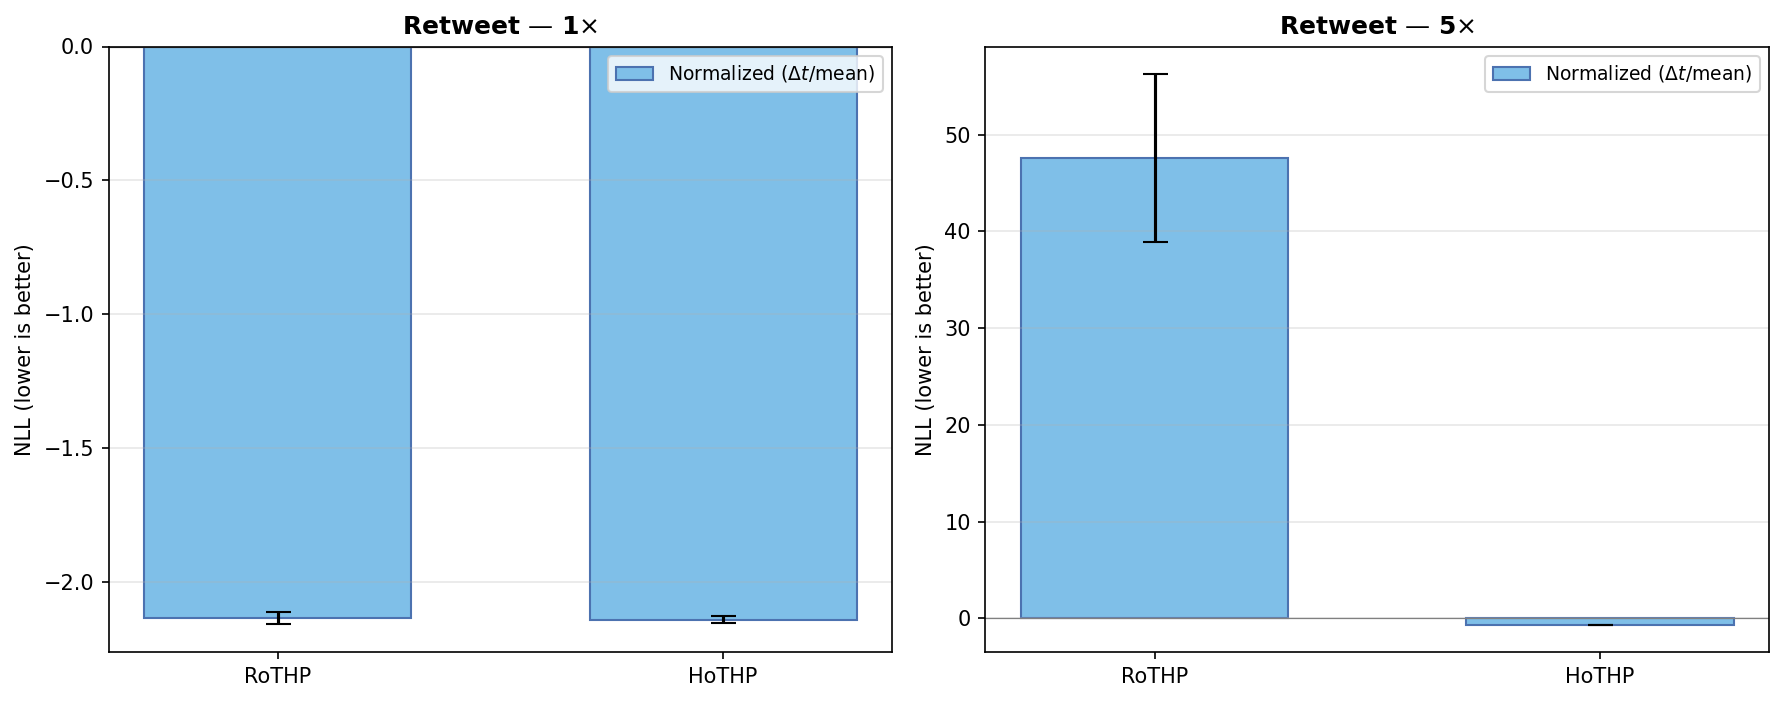
\includegraphics[width=14cm]{figuras/fig_ablacao_retweet_norm.png}
    }{
    }
\end{figure}

These results make it possible to separate the two factors that hurt the performance on Retweet. The primary problem was the numerical scale. The normalization benefits both models drastically. But even with the scale corrected, the HoTHP surpasses the RoTHP in extrapolation, confirming that the recency bias is advantageous on this dataset when the temporal scale allows its calibration. The residual instability of the RoTHP (with one seed still exploding at $5\times$) reinforces the fragility of the oscillatory kernel in extrapolation, also observed in the synthetic data.

\section{Discussion}
\label{sec:discussao-resultados}

The results on real data show that the recency bias of the HoTHP is beneficial in some scenarios and neutral or harmful in others. The analysis of the learned intensities suggests that the determining factor is not whether the process is self-exciting or self-inhibiting, but whether recent events are more informative than distant ones for the construction of the hidden state.

On Amazon, where the HoTHP obtains the best result, the process is self-inhibiting: the intensity grows with the time since the last event. Even so, the recency bias helps, because the immediately previous event is the most relevant for predicting the next one. The exponential decay in the attention correctly captures this relationship of decreasing relevance.

On Stackoverflow, where the three models tie, the intensity is practically constant. This indicates a process with little or no temporal memory, in which all the past events are equally (little) informative. The recency bias of the HoTHP does not significantly hurt (the constant intensity shows that the model manages to compensate in the intensity layer), but it also does not help, because there is no temporal structure to exploit.

On Retweet, the problem is twofold: the extreme temporal scale causes numerical collapse, and the structure of viral cascades may not align with the exponential decay. The ablation in Section~\ref{sec:ablacao-retweet} separated these two factors and showed that the primary problem was the scale: with normalization, the HoTHP obtains the best result of the whole benchmark (NLL $5\times = -0{,}542$), with almost zero variance between seeds. The RoTHP, even with normalization, still shows instability in the extrapolation, with one seed reaching NLL $= 255{,}9$.

The HoTHP proves more effective when two conditions are satisfied at the same time: (i) the process has short-range temporal memory, so that recent events are more informative than distant ones; and (ii) the scale of the intervals between events allows the parameter $\theta'$ to be calibrated properly during training, without numerical saturation. The Retweet ablation confirms that condition (ii) can be solved by preprocessing, and when it is, the recency bias of the HoTHP proves consistently advantageous.

\subsection{Computational cost versus benefit in extrapolation}
\label{subsec:custo-beneficio}

The hyperbolic kernel of the HoTHP involves more operations than the trigonometric kernel of the RoTHP, which is reflected in the training time. Table~\ref{tab:tempo-treino} presents the average training times (100 epochs, 3 seeds) for each combination of dataset and model.

\begin{table}[h!]
\centering
\caption{Average training time (minutes, 3 seeds). The factor indicates how many times slower the HoTHP is than the RoTHP.}
\label{tab:tempo-treino}
\begin{tabular}{lccc}
\toprule
Dataset & RoTHP (min) & HoTHP (min) & Factor \\
\midrule
Stackoverflow  &  2,4 &  3,1 & $1{,}26\times$ \\
Amazon         &  9,4 & 11,8 & $1{,}25\times$ \\
Taxi           &  1,9 &  2,0 & $1{,}05\times$ \\
Retweet (norm) & 43,5 & 97,6 & $2{,}24\times$ \\
\bottomrule
\end{tabular}
\end{table}

The overhead ranges from $1{,}05\times$ (Taxi) to $2{,}24\times$ (normalized Retweet), being more pronounced on datasets with long sequences, where the computation of the hyperbolic kernel dominates the time per batch. For datasets of moderate length (Stackoverflow, Amazon, Taxi), the additional cost is below $25\%$.

This cost, however, is paid only once during training. At inference time, the trained model is applied to sequences that are potentially much longer than the ones seen in training, exactly the extrapolation scenario. In this context, what matters is not the training speed, but whether the model produces valid results. The results in Table~\ref{tab:ablacao-retweet} illustrate the point clearly: on the normalized Retweet with $5\times$ extrapolation, the RoTHP obtains NLL $= 88{,}9 \pm 144{,}8$ (with one seed exploding to $255{,}9$), while the HoTHP obtains NLL $= -0{,}542 \pm 0{,}004$. Training the RoTHP $2{,}2\times$ faster only to then obtain unusable results in extrapolation does not constitute a practical advantage.
